\documentclass[11pt,a4paper]{article}

\usepackage[margin=2.2cm]{geometry}
\usepackage{amsmath,amssymb}
\usepackage{graphicx}
\usepackage{booktabs}
\usepackage{listings}
\usepackage{xcolor}
\usepackage[hidelinks]{hyperref}
\usepackage{caption}
\usepackage[section]{placeins}
\captionsetup{font=small,labelfont=bf}

\lstset{basicstyle=\ttfamily\small,columns=fullflexible,keepspaces=true,
        frame=single,rulecolor=\color{gray!50},xleftmargin=1em,xrightmargin=1em}
\newcommand{\code}[1]{\texttt{#1}}
\newcommand{\vx}{\mathbf{x}}

\title{Ear cutting on the sphere in glgrib\\[0.3em]
\large How \code{EarCut::processRing} triangulates coastline polygons, and how it converges}
\author{}
\date{2026-11-24}

\begin{document}
\sloppy
\maketitle

\begin{abstract}
glgrib fills land, lakes and Antarctic ice with triangles computed at start-up from the GSHHS
shapefiles. Each polygon (a \emph{ring}) is triangulated by an ear-cutting algorithm working
directly on the unit sphere, implemented in \code{src/glGrib/EarCut.cc}. This document describes
the algorithm and its data structures, then measures its convergence on the GSHHS data at three
resolutions, using a temporary instrumentation of the code. Each pass over a ring cuts 35--40\,\%
of its vertices at first, then 10--15\,\%; a land ring of $N$ vertices needs roughly
$\log N/\log(1/0.7)$ passes, and up to $\mathcal{O}(N)$ passes for thin river polygons.
The measurements also exposed two defects: the rotation that should move each ring to the equator
is applied transposed, which can break the spatial index and produce wrong triangles (Honshu at
intermediate resolution); and the OpenMP version can stop before a ring is finished.
\end{abstract}

\tableofcontents

%======================================================================
\section{Where ear cutting is used}

\code{Land::layer\_t::setup} (\code{src/glGrib/Land.cc}) reads a shapefile with
\code{ShapeLib::read}, which returns longitudes and latitudes in radians and a list of rings
separated by \code{OpenGL::restart}. \code{Land::layer\_t::triangulate} then:

\begin{enumerate}
\item computes the offset and length of every ring; the last point of a GSHHS ring repeats the
  first one and is dropped, so a ring of $N$ vertices has $N+1$ points in the file;
\item sorts the rings by decreasing size and reserves $3(N-2)$ indices per ring, the size of any
  triangulation of a simple polygon with $N$ vertices;
\item triangulates the rings of 300 vertices or more one after the other, with OpenMP used
  \emph{inside} \code{processRing} (\code{openmp = true});
\item triangulates the smaller rings in parallel, one ring per thread (\code{openmp = false}).
\end{enumerate}

\code{processRing} returns the number of indices actually written; when a ring is not completely
triangulated the remaining slots of its block are left unused. An optional subdivision step
(\code{Subdivide.cc}) then splits large triangles so that they follow the curvature of the sphere.

Table~\ref{tab:layers} lists the data. By default glgrib loads the crude (\code{c}) files of levels
1, 2, 3 and 5; the other resolutions are selected with \code{--land.layers[i].path}.

\begin{table}[!htb]
\centering\small
\begin{tabular}{lrrr}
\toprule
GSHHS level 1 (land) & rings & vertices & largest ring (Eurasia) \\
\midrule
crude (\code{c})        &     742 &      6\,540 &   1\,003 \\
intermediate (\code{i}) &  32\,830 &   307\,529 &  34\,331 \\
high (\code{h})         & 144\,749 & 1\,481\,718 & 139\,785 \\
\bottomrule
\end{tabular}
\caption{Size of the land layer at three resolutions. Levels 2 (lakes and river banks), 3
(islands in lakes), 5 and 6 (Antarctic ice front and grounding line) are triangulated the same way.}
\label{tab:layers}
\end{table}

%======================================================================
\section{The algorithm}

\subsection{Ear cutting in a nutshell}

A vertex $v$ of a simple polygon is an \emph{ear} when the triangle formed by $v$ and its two
neighbours lies inside the polygon. Cutting an ear outputs that triangle and removes $v$, leaving a
simple polygon with one vertex less; by the two-ears theorem (Meisters, 1975) every simple polygon
with more than three vertices has at least two ears, so repeating the operation $N-2$ times
triangulates the polygon. A vertex is an ear if and only if
\begin{itemize}
\item it is \emph{convex} (interior angle below $\pi$), and
\item no other vertex of the polygon lies inside its triangle. It is enough to test the
  \emph{reflex} vertices (interior angle above $\pi$): if a convex vertex's triangle contains a
  vertex, it contains a reflex one.
\end{itemize}
glgrib applies these tests on the unit sphere, where polygon edges are great-circle arcs, and
organises the work in \emph{passes}: each pass walks once around the ring and cuts every ear it
finds on its way.

\subsection{Change of frame (\code{getRotMat})}

\code{processRing} first converts the vertices to unit vectors $\vx_i$ and builds a frame in which
the ring should sit on the equator, far from the poles. With $w_i = \arccos(\vx_i\cdot\vx_{i+1})$
the length of edge $i$, normalised so that $\sum w_i = 1$:
\begin{align*}
\mathbf{r} &= \frac{\sum_i w_i \vx_i}{\|\sum_i w_i \vx_i\|}, &
\mathbf{s} &= \frac{\hat{\mathbf z}\times\mathbf r}{\|\hat{\mathbf z}\times\mathbf r\|}, &
\mathbf{t} &= \mathbf r\times\mathbf s,
\end{align*}
the vertices are projected on the plane $(\mathbf s,\mathbf t)$, $\xi_i=\mathbf s\cdot\vx_i$,
$\eta_i=\mathbf t\cdot\vx_i$, and the weighted covariance
\[
A = \sum_i w_i \begin{pmatrix}\xi_i^2 & \xi_i\eta_i\\ \xi_i\eta_i & \eta_i^2\end{pmatrix}
\]
is diagonalised in closed form (\code{Diag}). With $\mathbf q$ the eigenvector of the largest
eigenvalue, $\mathbf s' = q_1\mathbf s + q_2\mathbf t$ and $\mathbf t' = \mathbf r\times\mathbf s'$,
the function returns the matrix $R = [\mathbf r\;\mathbf s'\;\mathbf t']$ whose \emph{columns} are
the new axes. The intent is that the mean point $\mathbf r$ goes to longitude and latitude zero and
the long axis of the ring follows the equator, where longitude--latitude cells are least distorted.
The new coordinates are then $\lambda_i = \operatorname{atan2}(y_i, x_i)$,
$\varphi_i = \arcsin z_i$ with $(x_i,y_i,z_i) = R\,\vx_i$. Section~\ref{sec:rotation} shows that
this product should be $R^T\vx_i$.

For tiny rings ($|\det A| < 10^{-8}$) $R$ is the identity and the ring stays where it is.

\subsection{The ring as a doubly linked list (\code{node\_t})}

Each vertex is a \code{node\_t} holding its rank in the global array, its index in the ring, and
pointers to the previous and next vertex. Its angle is computed lazily and cached until a
neighbour changes (\code{dirty} flag). For vertex $j$ between $i$ and $k$:
\[
\mathbf u = \vx_j\times(\vx_i-\vx_j),\qquad
\mathbf w = \vx_j\times(\vx_k-\vx_j),\qquad
\theta_j = \operatorname{atan2}\bigl(\vx_j\cdot(\mathbf u\times\mathbf w),\;\mathbf u\cdot\mathbf w\bigr).
\]
$\mathbf u$ and $\mathbf w$ are tangent to the sphere at $\vx_j$ and normal to the two edges, so
$\theta_j\in(-\pi,\pi]$ is the signed angle between the edges. With the orientation of the GSHHS
rings (clockwise in longitude--latitude), a vertex is convex when $0<\theta_j<\pi$ and reflex when
$\theta_j<0$. Cutting an ear at $v$ reduces the interior angles of its two neighbours, so a convex
vertex never becomes reflex: the set of reflex vertices only shrinks.

\subsection{Point in spherical triangle (\code{inTriangle})}

For the triangle $(\mathbf t_0,\mathbf t_1,\mathbf t_2) = (\text{prev}, v, \text{next})$ and a
point $\mathbf p$:
\[
s_m = (\mathbf p - \mathbf t_m)\cdot\bigl(\mathbf t_m\times(\mathbf t_{m+1}-\mathbf t_m)\bigr)
    = \mathbf p\cdot(\mathbf t_m\times\mathbf t_{m+1}),\qquad m = 0,1,2.
\]
$s_m$ tells on which side of the plane of edge $m$ (a great circle) the point lies. The point is
inside when all non-zero $s_m$ have the same sign; a point exactly on an edge's great circle counts
as inside, which errs on the side of rejecting an ear.

\subsection{Spatial index of reflex vertices (\code{xy2node\_t})}

Testing every reflex vertex for every candidate ear would cost $\mathcal{O}(N^2)$ per pass. The
index splits the longitude--latitude box of the ring (in the rotated frame) into cells of about one
degree, $n_x = \max(2,\lfloor\Delta\lambda\rfloor)$ by $n_y = \max(2,\lfloor\Delta\varphi\rfloor)$
with $\Delta$ in degrees, and stores the reflex vertices of each cell in compressed form
(\code{off}, \code{len}, \code{nodes}). After each pass, \code{update} removes, cell by cell and
in parallel, the nodes that have been cut or have become convex. Nodes are never added, since no
vertex becomes reflex.

For a candidate ear, \code{begin} computes a search box:
\begin{itemize}
\item \textbf{latitude}: the range of the three edges. A great-circle arc can reach a higher or
  lower latitude than its end points; \code{getLatRange} parametrises the arc from $\vx_1$ to
  $\vx_2$ as $\vx(\theta) = \vx_1\cos\theta + \mathbf q\sin\theta$ with
  $\mathbf q = \mathbf p\times\vx_1$, $\mathbf p = \vx_1\times\vx_2/\|\vx_1\times\vx_2\|$, and
  checks the extrema of $z(\theta)$ at $\theta^* = \operatorname{atan2}(q_z, z_1)$ and
  $\theta^*+\pi$ when they fall inside the arc;
\item \textbf{longitude}: the union of the intervals spanned by the two edges at $v$, handled
  modulo $2\pi$ by \code{inter\_t}.
\end{itemize}
The iterator walks the cells of the box; only the vertices it returns are tested with
\code{inTriangle}.

\subsection{Passes (\code{earCut}) and termination}

One call to \code{earCut} is a pass:
\begin{lstlisting}
for (n = first; n != last; n = n->next)
  if (0 < angle (n) < pi && no reflex vertex of the index inside (prev, n, next))
    {
      output triangle (n, prev, next);
      n->cut (&n, ...);          // unlink n, continue from n->next
    }
\end{lstlisting}
After a cut the loop continues from the vertex that followed $n$, then advances once more, so
that vertex is skipped: two neighbouring vertices are never cut in the same pass, and a pass cuts
at most half of the vertices. Vertices cut during the pass stay in the index until the next
\code{update}.

\code{processRing} repeats passes until one leaves the vertex count unchanged:
\begin{lstlisting}
for (k = -1; ; )
  {
    earCut (...);  index.update ();
    count = ring.count ();
    if (count == k) break;
    k = count;
  }
\end{lstlisting}
A complete triangulation ends with two vertices and $N-2$ triangles.

\paragraph{OpenMP pools.} When \code{openmp} is true and the ring has more than 100 vertices, the
start of the list is moved 10 vertices forward and the ring is split into 8 chunks of
$c=\lfloor N/8\rfloor$ vertices. Pool $p$ walks from vertex $pc$ to vertex $(p+1)c-3$; the three
vertices left between two pools guarantee that two threads never modify the same links. Each pool
writes its triangles into its own vector; the vectors are concatenated at the end of the pass.
Figure~\ref{fig:pools} shows the first pass on Eurasia.

\begin{figure}[!htb]
\centering
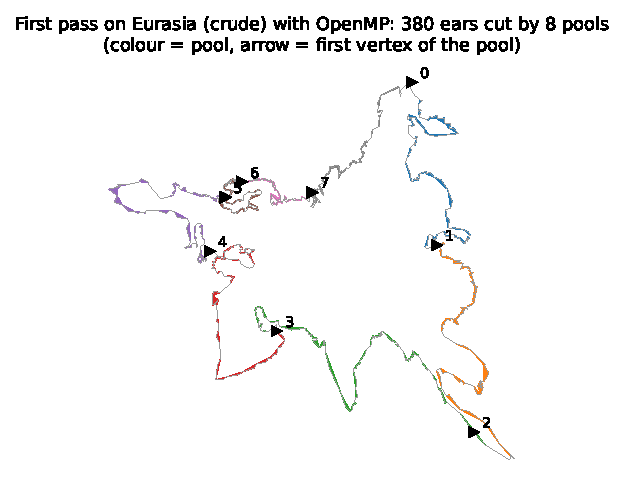
\includegraphics[width=0.8\textwidth]{fig/fig_openmp_pools.pdf}
\caption{First pass of the OpenMP version on Eurasia (crude, 1003 vertices). Each colour is a pool;
the pools work on 8 consecutive stretches of the coastline at the same time.}
\label{fig:pools}
\end{figure}

%======================================================================
\section{Convergence}

The figures in this section come from the instrumented code described in
Appendix~\ref{sec:repro}, with the rotation corrected to $R^T$ so that the defects of
Section~\ref{sec:defects} do not interfere. Unless stated otherwise the passes are serial.

\subsection{A pass at a time}

Figure~\ref{fig:australia} follows Australia (crude, 169 vertices) pass after pass. The first pass
removes the small teeth of the coastline: 64 of the 169 vertices (38\,\%). Each following pass
works on the polygon left by the previous one, whose edges are longer: the triangles grow from
pass to pass, and the last ones cross the whole continent. The reflex vertices disappear at the
same pace as the others (80 at the start, 12 after 5 passes), so the index empties and the ear
tests become cheaper. The last passes cut only a few ears each; 13 passes in all.

\begin{figure}[!htb]
\centering
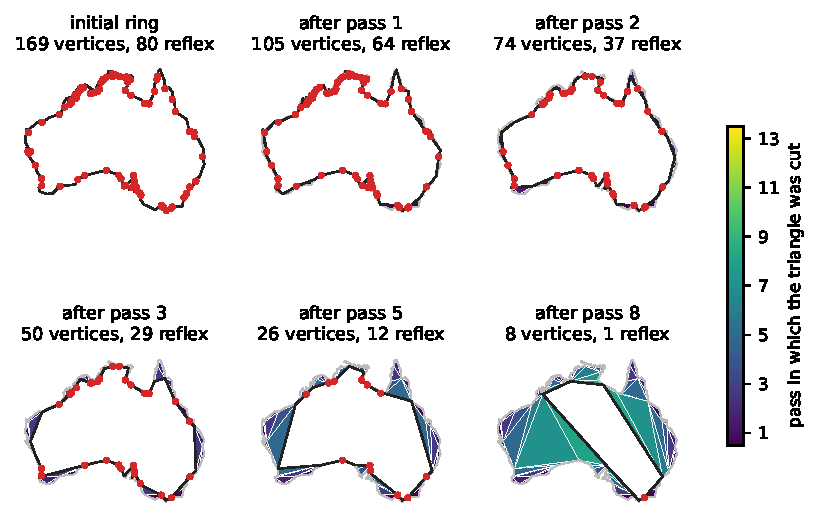
\includegraphics[width=\textwidth]{fig/fig_passes_australia.pdf}
\caption{Ear cutting on Australia (GSHHS crude, 169 vertices). Black: the ring that remains after
the pass; red dots: its reflex vertices; coloured triangles: those cut so far, coloured by pass.
All maps in this document use a gnomonic projection centred on the ring, in which great-circle
edges are straight lines.}
\label{fig:australia}
\end{figure}

The same layering is visible on whole continents (Figure~\ref{fig:bypass}): the first passes produce
slivers along the coast, the last ones a fan of large triangles in the interior.

\begin{figure}[!htb]
\centering
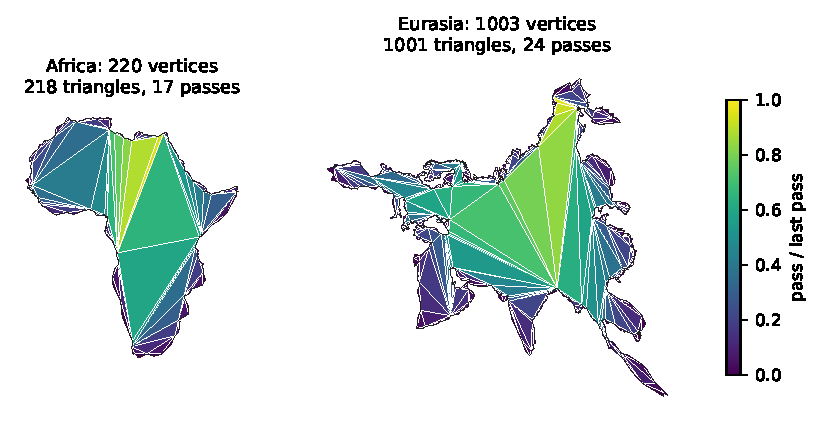
\includegraphics[width=\textwidth]{fig/fig_triangulation_by_pass.pdf}
\caption{Complete triangulations of Africa and Eurasia (crude), each triangle coloured by the pass
that cut it, relative to the last pass.}
\label{fig:bypass}
\end{figure}

\subsection{Rate of convergence}

Figure~\ref{fig:convergence} shows the number of vertices left after each pass for the largest
ring, Eurasia, at the three resolutions. The first pass removes 36--39\,\% of the vertices,
not far from the 50\,\% limit set by the skipped neighbour. The fraction then decreases to
10--15\,\% and stays there: the remaining polygon gets smoother, but its large-scale concavities
(seas, gulfs, peninsulas) remain and block many candidate ears. The decrease is therefore
geometric at an almost constant rate during most of the run, and the curves of the three
resolutions are nearly parallel on a logarithmic scale.

\begin{figure}[!htb]
\centering
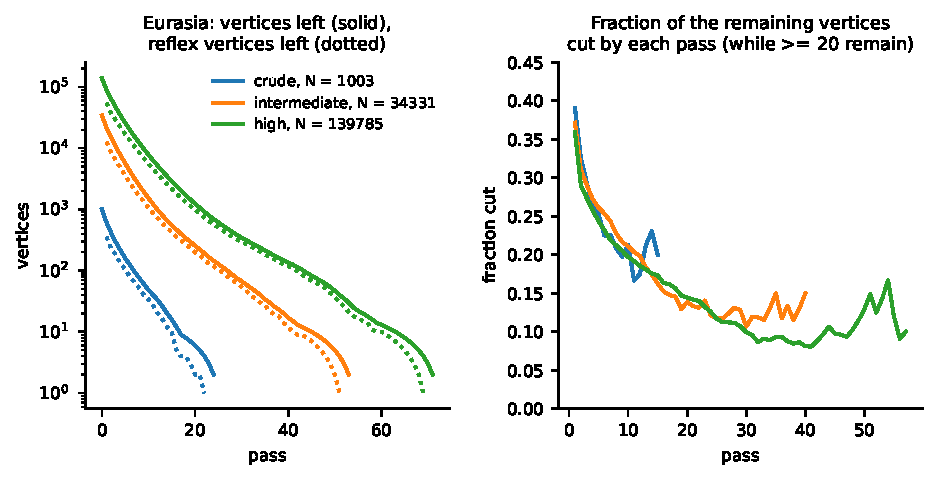
\includegraphics[width=\textwidth]{fig/fig_convergence.pdf}
\caption{Eurasia at three resolutions. Left: vertices (solid) and reflex vertices (dotted) left
after each pass. Right: fraction of the remaining vertices cut by each pass.}
\label{fig:convergence}
\end{figure}

\begin{table}[!htb]
\centering\small
\begin{tabular}{lrrr}
\toprule
Eurasia & $N$ & passes, serial & passes, OpenMP \\
\midrule
crude        &   1\,003 & 24 & 19 \\
intermediate &  34\,331 & 53 & 47 \\
high         & 139\,785 & 71 & 66 \\
\bottomrule
\end{tabular}
\caption{Passes that cut at least one ear, for the largest ring.}
\label{tab:passes}
\end{table}

With a constant fraction $f$ cut per pass, $N$ vertices need $\log N/\log(1/(1-f))$ passes.
Figure~\ref{fig:passesn} plots the number of passes against $N$ for every ring of the high
resolution data, with the curve for $f=0.3$:
\begin{itemize}
\item \textbf{Land (level 1).} The median follows $\log N$ up to a few thousand vertices; the
  largest rings need about twice as many passes as the model, because the fraction drops to
  10\,\% in their late passes. Eurasia needs 71 passes for 139\,785 vertices.
\item \textbf{Lakes and rivers (level 2).} Many rings need far more passes, up to several
  hundred. These are rivers stored as long thin polygons (Section~\ref{sec:river}).
\end{itemize}
The OpenMP version needs slightly fewer passes on large rings (Table~\ref{tab:passes}); the
reason was not investigated. Its outliers below the cloud on the right panel are rings where it stopped too early
(Section~\ref{sec:openmp}).

\begin{figure}[!htb]
\centering
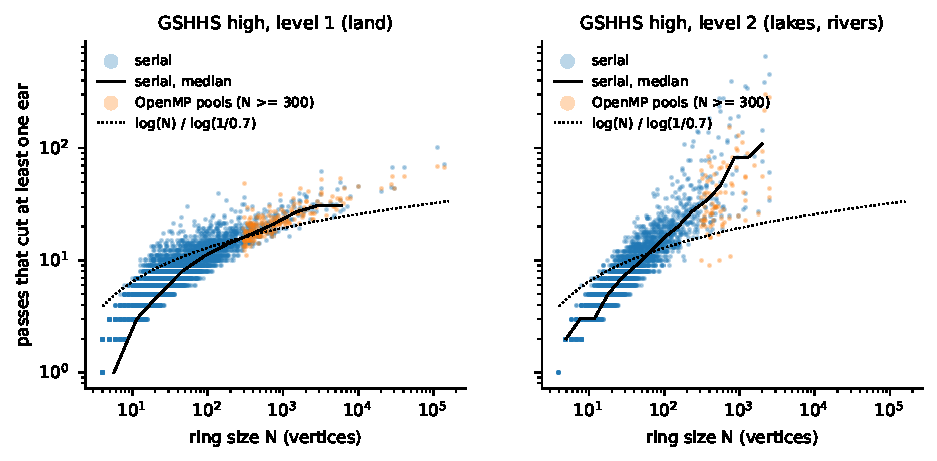
\includegraphics[width=\textwidth]{fig/fig_passes_vs_n.pdf}
\caption{Number of passes against ring size, GSHHS high resolution. Blue: serial; orange: OpenMP
pools (rings of 300 vertices or more, as in glgrib); black: median of the serial runs; dotted:
$\log N/\log(1/0.7)$.}
\label{fig:passesn}
\end{figure}

\subsection{Worst case: thin polygons}
\label{sec:river}

Level 2 stores the large rivers as polygons that follow both banks. Figure~\ref{fig:river} shows the
Ob and the Irtysh (intermediate, 811 vertices). After the first pass has removed the small
wiggles, nearly every convex vertex sees a reflex vertex of the opposite bank inside its triangle,
and only a few ears exist at any time (two, in the state where the OpenMP version stops). The serial version needs 392 passes, cutting about
two ears per pass: the number of passes grows like $N$ instead of $\log N$. Ear cutting by passes
gives no guarantee better than $\mathcal{O}(N)$ passes, and each pass costs $\mathcal{O}(N)$ for
the walk around the ring.

\begin{figure}[!htb]
\centering
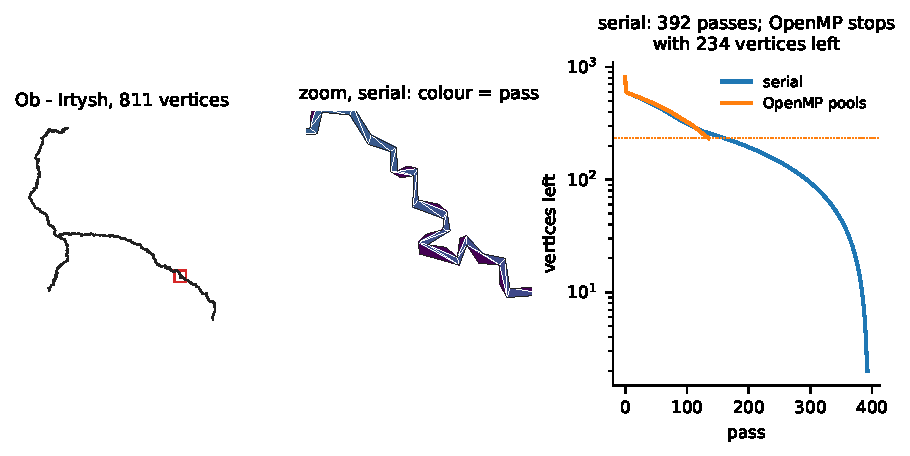
\includegraphics[width=\textwidth]{fig/fig_river.pdf}
\caption{The Ob--Irtysh river polygon (GSHHS intermediate, level 2). Middle: zoom on the red box,
triangles coloured by pass. Right: vertices left after each pass; the OpenMP version stops with
234 vertices left (Section~\ref{sec:openmp}).}
\label{fig:river}
\end{figure}

\subsection{Cost}

Measured with the stand-alone driver (Appendix~\ref{sec:repro}) on 14 cores, without
instrumentation output, on the high-resolution land layer:

\begin{center}\small
\begin{tabular}{lrr}
\toprule
 & serial & OpenMP pools \\
\midrule
Eurasia (139\,785 vertices)        & 0.31\,s & 0.11\,s \\
North America (111\,435 vertices)  & 0.30\,s & 0.10\,s \\
whole layer (144\,749 rings)       & 2.9\,s  & 2.2\,s \\
\bottomrule
\end{tabular}
\end{center}

In the whole-layer runs the driver handles the small rings one after the other; glgrib runs them
in parallel.

%======================================================================
\section{Defects found}
\label{sec:defects}

Table~\ref{tab:failures} counts the rings left incomplete, over all GSHHS files in
\code{share/glgrib/coastlines/shp}. Files not listed (all crude and low resolution files, levels
3 and 5, level 1 at high resolution, level 6 at intermediate resolution) have none. None of the
crude files that glgrib loads by default is affected.

\begin{table}[!htb]
\centering\small
\begin{tabular}{lrcccc}
\toprule
file & rings & as in glgrib & with $R^T$ & serial & serial with $R^T$ \\
\midrule
\code{GSHHS\_i\_L1} & 32\,830 & 2 & 1 & 2 & 1 \\
\code{GSHHS\_i\_L2} &  6\,559 & 4 & 4 & 1 & 1 \\
\code{GSHHS\_h\_L2} &  6\,601 & 13 & 13 & 0 & 0 \\
\code{GSHHS\_h\_L6} &     345 & 1 & 1 & 1 & 1 \\
\bottomrule
\end{tabular}
\caption{Rings left incomplete. ``As in glgrib'': OpenMP pools for rings of 300 vertices or more,
rotation $R$. The rings that remain in the last column have invalid geometry
(Section~\ref{sec:input}).}
\label{tab:failures}
\end{table}

\subsection{The rotation is applied transposed}
\label{sec:rotation}

\code{getRotMat} returns $R=[\mathbf r\;\mathbf s'\;\mathbf t']$ with the new axes as columns
(\code{glm::mat3} is column-major), and \code{processRing} computes
\begin{lstlisting}
xyz2[i] = R * xyz1[i];
\end{lstlisting}
The coordinates of $\vx$ in the new frame are $(\mathbf r\cdot\vx,\mathbf s'\cdot\vx,
\mathbf t'\cdot\vx) = R^T\vx$, not $R\vx$. Fitting the matrix from the dumped coordinates confirms
it: $R^T$ sends the mean point of every ring to $(1,0,0)$, $R$ sends it anywhere. With $R$ the
rings are rotated to arbitrary places, sometimes next to a pole (Figure~\ref{fig:rotation}):
Eurasia crosses the date line and reaches 88$^\circ$, Honshu lands on the South Pole.

\begin{figure}[!htb]
\centering
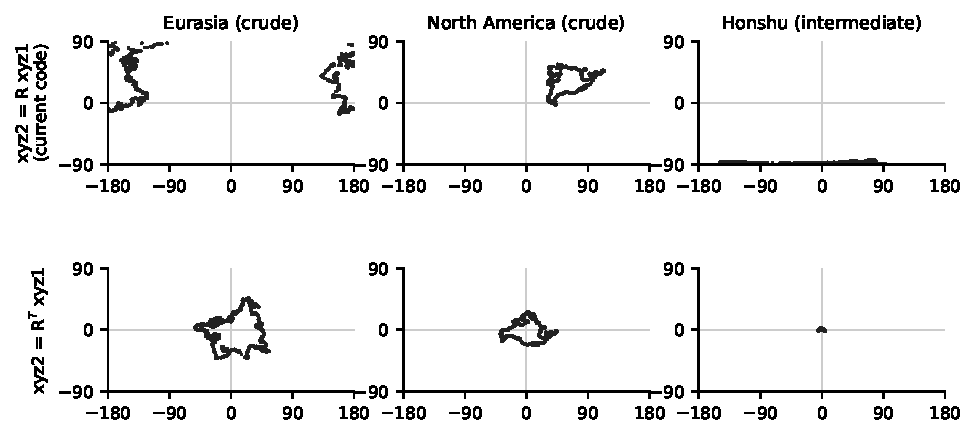
\includegraphics[width=\textwidth]{fig/fig_rotation.pdf}
\caption{Vertices of three rings in the frame used by the algorithm. Top: current code; bottom:
with the transposed matrix, each ring centred at $(0,0)$ along the equator.}
\label{fig:rotation}
\end{figure}

Near a pole the longitude--latitude index degenerates, and a chain of three problems leads to a
wrong triangle on Honshu (intermediate resolution, 1541 vertices):
\begin{enumerate}
\item The ring surrounds the pole in the rotated frame, so its longitude range exceeds $2\pi$.
  \code{getLonRange} returns $\lambda_{\min} > \lambda_{\max}$ and $n_x$ is computed from the
  negative difference before the range is unwrapped: the index gets $n_x = 2$ columns of
  $4.2$ radians instead of about 360 cells of one degree.
\item The search box of ear $(779, 786, 791)$ runs from $3.725$ to $3.785$ radians, across the
  seam of the index range $[-4.72, 3.75]$; after wrapping, \code{ixmin = 1} and \code{ixmax = 0}.
\item The iterator computes \code{nx = ixmax - ixmin + 1 = 0} and does not wrap around, so it
  never visits column 0, where reflex vertex 792 is stored.
\end{enumerate}
Vertex 792 lies inside the triangle; the test that would reject the ear is never made. Pass 4 cuts
the ear, the triangles overlap, the remaining polygon turns inside out and the algorithm stops with
four reflex vertices (Figure~\ref{fig:honshu}). A trace of the ear test (instrumentation variable
\code{GLGRIB\_EARCUT\_DEBUG}) shows the iterator returning 63 candidates, none of them 792, while
\code{inTriangle} reports 792 inside.

\begin{figure}[!htb]
\centering
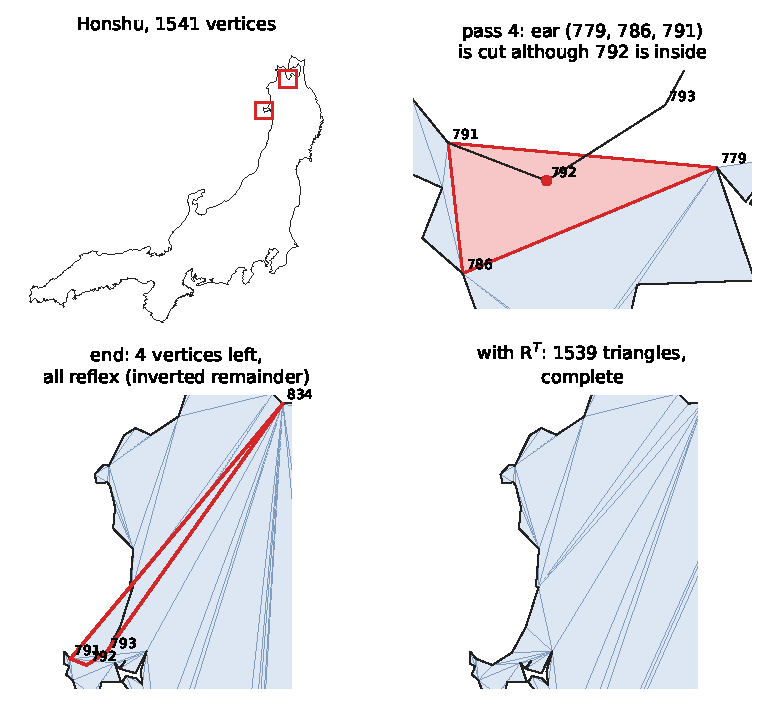
\includegraphics[width=0.85\textwidth]{fig/fig_failure_honshu.pdf}
\caption{Honshu, GSHHS intermediate. The ear $(779, 786, 791)$ is cut although reflex vertex 792 is
inside, because the index search misses it. With $R^T$ the ring stays near the equator, the index
is regular and the triangulation completes.}
\label{fig:honshu}
\end{figure}

With $R^T$ every ring is centred on $(0,0)$ and only a ring spanning about $180^\circ$ of
longitude would reach the seam; all rings tested are then triangulated, except the invalid ones of
Section~\ref{sec:input}. The index problems remain in the code, though, and would come back for
such a ring.

\subsection{The OpenMP version can stop too early}
\label{sec:openmp}

A pool walks from its first vertex to three vertices before the next pool; the last pool stops
three vertices before the end of the list. In every pass, $3\times8$ vertices plus a few at the end
are never examined. The loop in \code{processRing} stops as soon as a pass cuts nothing. When the
only ears of the ring sit in these unexamined places, the loop stops on an unfinished ring.

This happens on rings with few ears, the river polygons of level 2. On the Ob--Irtysh
(Figure~\ref{fig:river}), the OpenMP version stops after 135 passes with 234 vertices left; the
remaining polygon still has two valid ears (vertices 331 and 653), which a serial pass would have
cut. The serial version, which examines every vertex but the last one, completes all rings of
level 2 at high resolution where the OpenMP version leaves 13.

\subsection{Invalid input}
\label{sec:input}

Three rings cannot be triangulated by any variant, because their geometry is not a simple
polygon on the sphere:
\begin{itemize}
\item ring 194020 of \code{GSHHS\_i\_L1} (19 vertices, Maine) intersects itself twice
  (Figure~\ref{fig:selfint});
\item ring 81960 of \code{GSHHS\_i\_L2} has four vertices, two of them $10^{-6}$ radians apart:
  one triangle of zero area is missing;
\item ring 17477 of \code{GSHHS\_h\_L6} (West Antarctica, 18\,898 vertices) goes through the South
  Pole twice, as $(0^\circ,-90^\circ)$ and $(-180^\circ,-90^\circ)$, two coincident points on the
  sphere; 24 triangles are missing.
\end{itemize}

\begin{figure}[!htb]
\centering
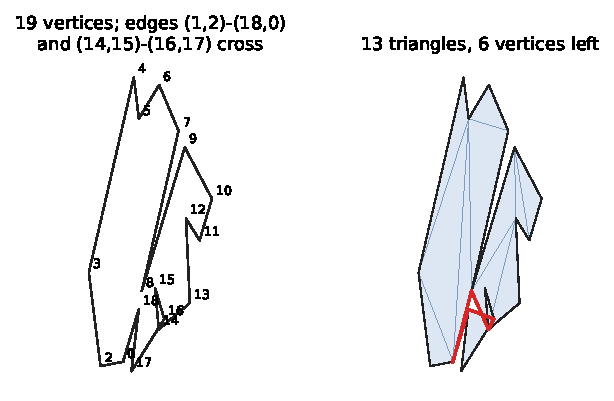
\includegraphics[width=0.75\textwidth]{fig/fig_selfintersect.pdf}
\caption{A self-intersecting ring (GSHHS intermediate, level 1). Ear cutting stops with six
vertices left (red).}
\label{fig:selfint}
\end{figure}

\subsection{Minor issues}

\begin{itemize}
\item \code{xy2ind (int, int)} wraps with \code{while (ix > nx)}; it should be \code{ix >= nx}.
\item The latitude bounds of the index are clipped to $\pm\pi$ instead of $\pm\pi/2$.
\item In \code{getLatRange (nodevec, ...)} the first loop is overwritten by the second and has no
  effect.
\item The serial pass runs from the first vertex to its predecessor and never examines the
  predecessor itself.
\item The angle and the point-in-triangle test are computed in single precision. A vertex where
  the ring goes straight on has $\theta\approx\pm\pi$, and rounding can classify it either way; one
  such degenerate triangle was found on Honshu.
\end{itemize}

\subsection{Possible fixes}

Not applied; listed for reference.
\begin{enumerate}
\item In \code{processRing}: \code{xyz2[i] = glm::transpose (R) * xyz1[i];}.
\item In \code{xy2node\_t}: compute \code{nx} after unwrapping the longitude range, and in the
  iterator, when \code{ixmax < ixmin}, add the number of columns to \code{ixmax} so that the walk
  wraps through \code{xy2ind (int, int)}.
\item In \code{processRing}: when a pass with OpenMP pools cuts nothing, run one serial pass
  before giving up; or let the pools start at a different offset from one pass to the next and
  stop only after a serial pass has failed.
\end{enumerate}

%======================================================================
\appendix
\section{Reproducing the measurements}
\label{sec:repro}

The files are in \code{share/doc/earcut/tools}:
\begin{description}
\item[\code{earcut-instrumentation.patch}] temporary changes to \code{src/glGrib/EarCut.cc}, all
  marked \code{EARCUT\_DUMP}. They are driven by environment variables:
  \code{GLGRIB\_EARCUT\_DUMP=dir} writes one line per ring (size, triangles, vertices and reflex
  vertices left after each pass) to \code{dir/stats.txt};
  \code{GLGRIB\_EARCUT\_DUMP\_MIN=N} also writes \code{dir/ring\_<rank>.txt}, with the
  coordinates of the ring and the triangles cut by each pass, for rings of $N$ vertices or more;
  \code{GLGRIB\_EARCUT\_NOOMP=1} forces the serial version;
  \code{GLGRIB\_EARCUT\_FIXROT=1} applies $R^T$ instead of $R$;
  \code{GLGRIB\_EARCUT\_DEBUG=j} traces the ear test of vertex $j$.
\item[\code{earcut\_driver.cc}] reads a GSHHS shapefile into rings exactly as
  \code{ShapeLib::read} and \code{Land::layer\_t::triangulate} do (same ranks, same lengths, OpenMP
  only for rings of 300 vertices or more) and calls \code{EarCut::processRing}. Selected rings give
  the same results as inside glgrib, in a fraction of a second.
\item[\code{ring.py}, \code{figs.py}] read the dumps and draw the figures.
\item[\code{make-figures.sh}] builds the driver against the instrumented \code{EarCut.cc}, produces
  the dumps and runs \code{figs.py}.
\end{description}
\begin{lstlisting}
git apply share/doc/earcut/tools/earcut-instrumentation.patch
cd share/doc/earcut && ./tools/make-figures.sh /tmp/earcut
cd ../../.. && git checkout src/glGrib/EarCut.cc
pdflatex earcut.tex; pdflatex earcut.tex
\end{lstlisting}

Ring ranks are offsets in the vertex array of a layer; the rings used in the figures are 2230
(Australia), 1031 (Africa), 0 (Eurasia) and 1252 (North America) in \code{GSHHS\_c\_L1}, 102218
(Honshu) and 194020 in \code{GSHHS\_i\_L1}, and 87722 (Ob--Irtysh) in \code{GSHHS\_i\_L2}.

\end{document}
